%\renewcommand{\theequation}{\theenumi}
%\begin{enumerate}[label=\arabic*.,ref=\thesubsection.\theenumi]
%\numberwithin{equation}{enumi}
    \item Solve $30x < 200$ when
    \begin{enumerate} 
    \item  x is a natural number,
    \item x is an integer.
\end{enumerate}
\solution From the given information, 
\begin{align}
30x < 200 \implies x < \frac{20}{3}
\label{eq:lineq_nat}
\end{align}
If $x$ is a natural number, $x \in \cbrak{1, 2, 3, 4, 5, 6}$. If $x$ is an integer, then the solution set includes 0 as well as all negative integers.
    \item Solve $5x-3 < 3x+1$ when
    \begin{enumerate} 
\item  x is an integer,
    \item x is a real number.
\end{enumerate}
\solution 
\begin{align}
5x-3 < 3x+1 \implies x < 2
\label{eq:lineq_real}
\end{align}
%
If $x$ is real, then $x \in \brak{-\infty, 2}$. 
%Fig.  provides a graphical solution using the following python code
%\begin{lstlisting}
%\end{lstlisting}
    \item Solve the following system of linear inequalities graphically.
\begin{align}
\label{eq:line_two_ineq}
\begin{split}
    x+y &\geq 5
\\
    x-y &\leq 3
\end{split}
\end{align}
\solution  Let $u_1 \ge 0, u_2 \ge 0$.  This may be expressed as
\begin{align}
\vec{u} = \myvec{u_1\\u_2}\succeq \vec{0}
\end{align}
%
\eqref{eq:line_two_ineq} can then be expressed as
\begin{align}
\begin{split}
    x+y &\geq 5
\\
    -x+y &\geq -3
\end{split}
%
\\
\implies 
\myvec{1 & 1 \\ -1 & 1}\vec{x}  &\succeq \myvec{5\\-3}
\\
\myvec{1 & 1 \\ -1 & 1}\vec{x}  -\vec{u}&=\myvec{5\\-3}
\\
\text{or, }
\myvec{1 & 1 \\ -1 & 1}\vec{x} &= \myvec{5\\-3} +\vec{u}
\end{align}
%
resulting in 
\begin{align}
\vec{x} &= \myvec{1 & 1 \\ -1 & 1}^{-1}\myvec{5\\-3} +\myvec{1 & 1 \\ -1 & 1}^{-1}\vec{u}
\\
\text{or, } \vec{x} &= \myvec{4\\1} +\frac{1}{2}\myvec{1 & -1 \\ 1 & 1}\vec{u}
\end{align}
%
after obtaining the  inverse.
%
 Fig. \ref{fig:line_ineq} generated using the following python code shows the region satisfying \eqref{eq:line_two_ineq}

\begin{lstlisting}
codes/line/line_ineq.py
\end{lstlisting}
%
\begin{figure}[!ht]
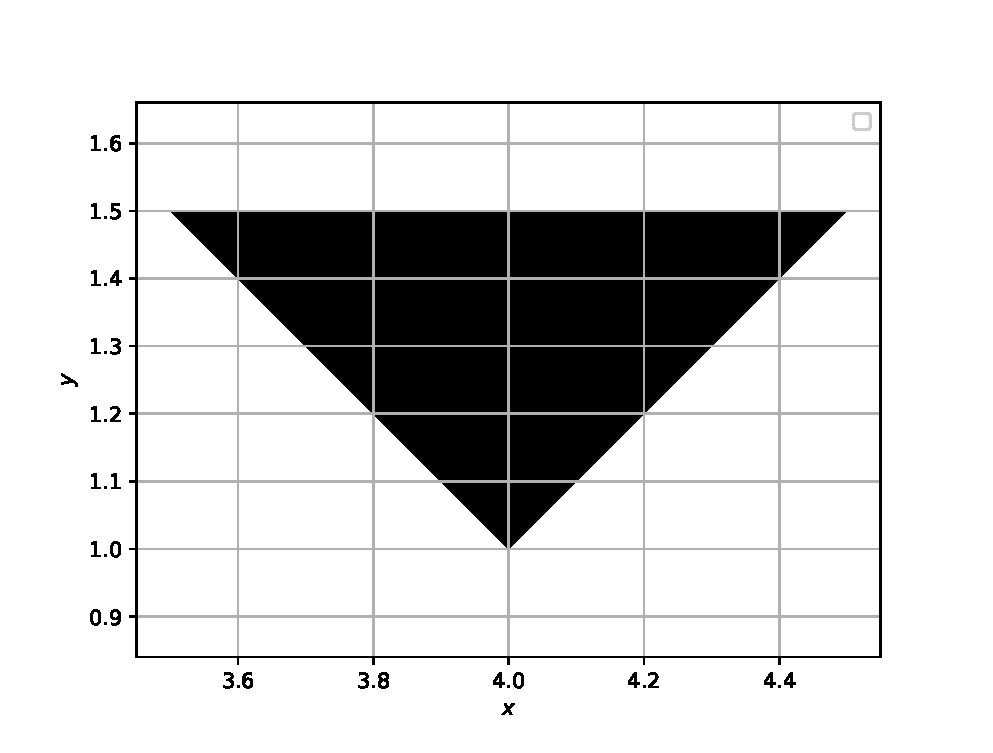
\includegraphics[width=\columnwidth]{./line/figs/line_ineq.eps}
\caption{}
\label{fig:line_ineq}
\end{figure}
%
\item Solve 
\begin{align}
\begin{split}
2x+y \geq 4
\\ 
x+y \leq 3
\\ 
2x-3y \leq 6
\end{split}
\label{eq:line_mult_ineq}
\end{align}
%
\\
\solution  Fig. \ref{fig:line_ineq_mult} generated using the following python code shows the region satisfying \eqref{eq:line_mult_ineq}

\begin{lstlisting}
codes/line/line_ineq_mult.py
\end{lstlisting}
%
\begin{figure}[!ht]
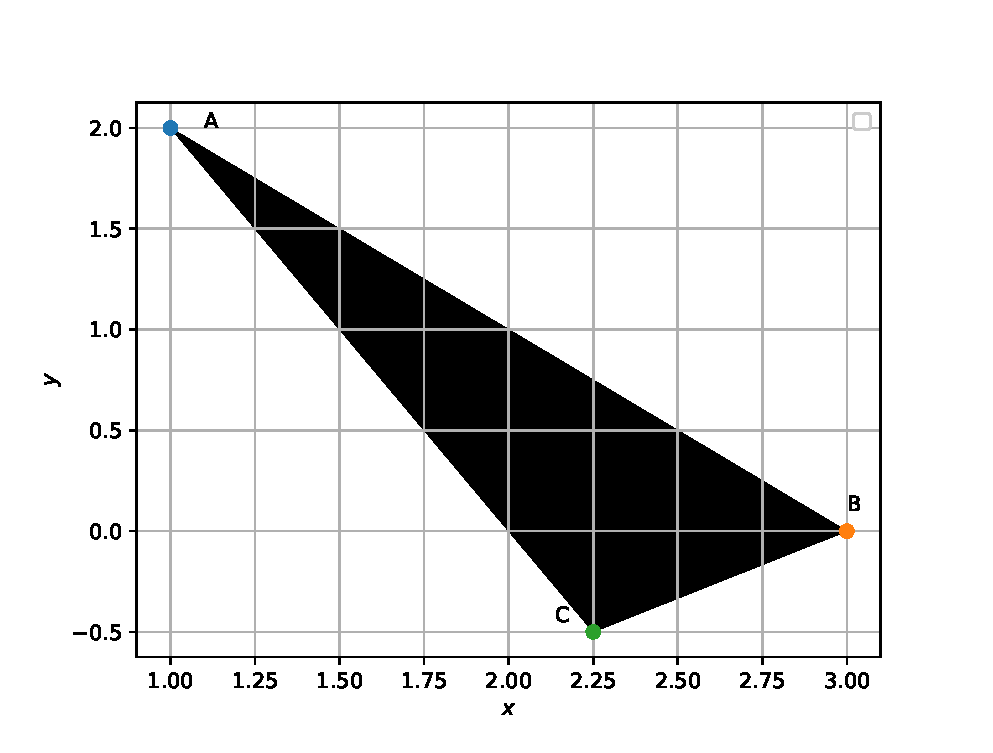
\includegraphics[width=\columnwidth]{./line/figs/line_ineq_mult.eps}
\caption{}
\label{fig:line_ineq_mult}
\end{figure}
%
\item   Solve    $x+y < 5$ graphically.
\\
\solution 
The following python code generates Fig. \ref{fig:3.11.5_qsix}.
	\begin{lstlisting}
	./solutions/5/codes/lines/q6.py
	\end{lstlisting}
	\begin{figure}[!ht]
	\centering
	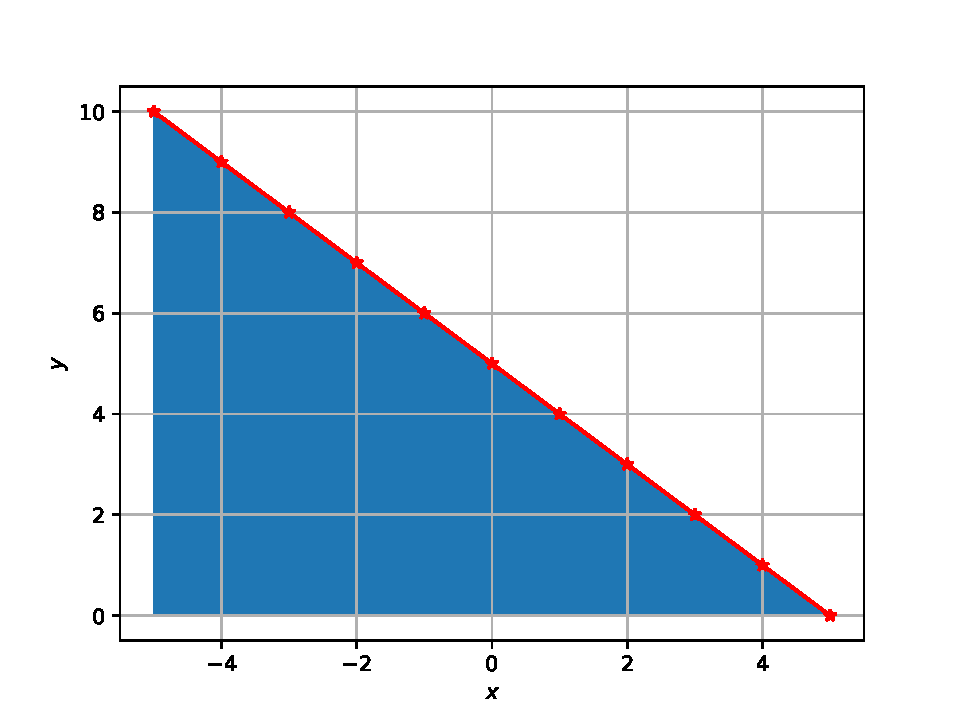
\includegraphics[width=\columnwidth]{./solutions/5/figs/lines/q6.eps}
	\caption{x+y$<$5}
	\label{fig:3.11.5_qsix}	
	\end{figure}
	

%
    \item Solve 
\begin{align}
\myvec{3 & 2 \\ 1 & 4 \\ 1 & 0 \\ 0 & -1 \\ -1 & 0} \vec{x}\preceq \myvec{150\\80\\15\\0\\0}
%3x+2y \leq 150
%\\ 
%x+4y \leq 80
%\\ 
%x \leq 15
%\\ 
%y \geq 0
%\\
%x \geq 0 
\end{align}
%
   
%    \end{enumerate}
\item Solve  x $\geq$ 3, y $\geq$ 2 graphically.
\\
\solution 
The given curve 
\begin{align}
	y =\frac{1}{x-1}
\end{align}
can be expressed as 
\begin{align}
	xy - y - 1 = 0 \label{eq:solutions/1/14/eq:hyperbola}
\end{align}
Hence, we have
\begin{align}
	\vec{V} = \frac{1}{2}\myvec{0 & 1 \\ 1 & 0}, 
	\vec{u} = \frac{1}{2}\myvec{0 \\-1},
	f = -1
\end{align}
Since $\mydet{\vec{V}} < 0$, the equation \eqref{eq:solutions/1/14/eq:hyperbola} represents hyperbola.
To find the values of $\lambda_1$ and $\lambda_2$, consider the characteristic equation,
\begin{align}
	\mydet{\lambda\vec{I} - \vec{V}} &= 0\\
	\implies \mydet{\myvec{\lambda & 0\\0 & \lambda} - \myvec{0 & \frac{1}{2} \\ \frac{1}{2} & 0}} &= 0\\
	\implies \mydet{ \lambda & \frac{-1}{2} \\ \frac{-1}{2} & \lambda} &= 0\\
	\implies \lambda_1 &= \frac{1}{2} , \lambda_2 = \frac{-1}{2}
\end{align}
In addition, given the slope -1, the direction and normal vectors are given by 
\begin{align}
	\vec{m} = \myvec{1 \\ -1} \\
	\vec{n} = \myvec{ 1 \\ 1}
\end{align}
The parameters of hyperbola are as follows:
\begin{align}
	\vec{c} &= -\vec{V}^{-1}\vec{u} \\
	&= -\myvec{0 & 2\\ 2 & 0}\myvec{0 \\ -\frac{1}{2}} \\
	&= \myvec{1 \\ 0}\\
	axes &= \begin{cases}
	\sqrt{\frac{\vec{u}^T\vec{V}^{-1}\vec{u} - f}{\lambda_1}} = \sqrt{2}\\
 \sqrt{\frac{f-\vec{u}^T\vec{V}^{-1}\vec{u}}{\lambda_2}} = \sqrt{2}
\end{cases}
\end{align}
which represents the standard hyperbola equation,
\begin{align}
	\frac{x^2}{2} - \frac{x^2}{2} = 1
\end{align}
The points of contact are given by 
\begin{align}
  \tiny{K} &=\pm \sqrt{\frac{\vec{u}^T\vec{V}^{-1}\vec{u} - f}{\vec{n}^T\vec{V}^{-1}\vec{n}}}
  = \pm \frac{1}{2}\\
  \vec{q} &= \vec{V}^{-1}(k\vec{n}-\vec{u})\\
  \vec{q_1} &= \myvec{0 & 2\\2 & 0} \sbrak{\frac{1}{2}\myvec{1 \\ 1} - \myvec{0\\ \frac{-1}{2}}}\\
  &= \myvec{2 \\ 1}\\
  \vec{q_2} &= \myvec{0 & 2\\2 & 0} \sbrak{\frac{-1}{2}\myvec{1 \\ 1} - \myvec{0\\ \frac{-1}{2}}}\\
  &= \myvec{0 \\ -1}
\end{align} 
$\therefore$ The tangents are given by
\begin{align}
	\myvec{1 & 1} \brak{\vec{x} - \myvec{2 \\ 1}} = 0 \\
	\myvec{1 & 1} \brak{\vec{x} - \myvec{0 \\ -1}} = 0
\end{align}
The desired equations of all lines having slope -1 that are tangents to the curve $\frac{1}{x-1}, x \neq 1$ are given by
\begin{align}
	\myvec{1 & 1}\vec{x} &= 3 \\
	\myvec{1 & 1}\vec{x} &= -1 
\end{align}
The above results are verified in the following figure.
\begin{figure}[h!] \label{eq:solutions/1/14/fig:tangents}
	\centering
	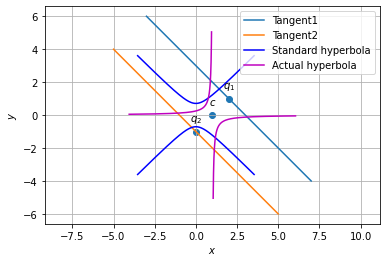
\includegraphics[width=\columnwidth]{./solutions/1/14/graph7.png}
	\caption{The standard and actual hyperbola.}
\end{figure}


    \item Solve 7x+3 $<$ 5x+9. Show the graph of the solutions on number line.
\\
\solution 
The given curve 
\begin{align}
	y =\frac{1}{x-1}
\end{align}
can be expressed as 
\begin{align}
	xy - y - 1 = 0 \label{eq:solutions/1/14/eq:hyperbola}
\end{align}
Hence, we have
\begin{align}
	\vec{V} = \frac{1}{2}\myvec{0 & 1 \\ 1 & 0}, 
	\vec{u} = \frac{1}{2}\myvec{0 \\-1},
	f = -1
\end{align}
Since $\mydet{\vec{V}} < 0$, the equation \eqref{eq:solutions/1/14/eq:hyperbola} represents hyperbola.
To find the values of $\lambda_1$ and $\lambda_2$, consider the characteristic equation,
\begin{align}
	\mydet{\lambda\vec{I} - \vec{V}} &= 0\\
	\implies \mydet{\myvec{\lambda & 0\\0 & \lambda} - \myvec{0 & \frac{1}{2} \\ \frac{1}{2} & 0}} &= 0\\
	\implies \mydet{ \lambda & \frac{-1}{2} \\ \frac{-1}{2} & \lambda} &= 0\\
	\implies \lambda_1 &= \frac{1}{2} , \lambda_2 = \frac{-1}{2}
\end{align}
In addition, given the slope -1, the direction and normal vectors are given by 
\begin{align}
	\vec{m} = \myvec{1 \\ -1} \\
	\vec{n} = \myvec{ 1 \\ 1}
\end{align}
The parameters of hyperbola are as follows:
\begin{align}
	\vec{c} &= -\vec{V}^{-1}\vec{u} \\
	&= -\myvec{0 & 2\\ 2 & 0}\myvec{0 \\ -\frac{1}{2}} \\
	&= \myvec{1 \\ 0}\\
	axes &= \begin{cases}
	\sqrt{\frac{\vec{u}^T\vec{V}^{-1}\vec{u} - f}{\lambda_1}} = \sqrt{2}\\
 \sqrt{\frac{f-\vec{u}^T\vec{V}^{-1}\vec{u}}{\lambda_2}} = \sqrt{2}
\end{cases}
\end{align}
which represents the standard hyperbola equation,
\begin{align}
	\frac{x^2}{2} - \frac{x^2}{2} = 1
\end{align}
The points of contact are given by 
\begin{align}
  \tiny{K} &=\pm \sqrt{\frac{\vec{u}^T\vec{V}^{-1}\vec{u} - f}{\vec{n}^T\vec{V}^{-1}\vec{n}}}
  = \pm \frac{1}{2}\\
  \vec{q} &= \vec{V}^{-1}(k\vec{n}-\vec{u})\\
  \vec{q_1} &= \myvec{0 & 2\\2 & 0} \sbrak{\frac{1}{2}\myvec{1 \\ 1} - \myvec{0\\ \frac{-1}{2}}}\\
  &= \myvec{2 \\ 1}\\
  \vec{q_2} &= \myvec{0 & 2\\2 & 0} \sbrak{\frac{-1}{2}\myvec{1 \\ 1} - \myvec{0\\ \frac{-1}{2}}}\\
  &= \myvec{0 \\ -1}
\end{align} 
$\therefore$ The tangents are given by
\begin{align}
	\myvec{1 & 1} \brak{\vec{x} - \myvec{2 \\ 1}} = 0 \\
	\myvec{1 & 1} \brak{\vec{x} - \myvec{0 \\ -1}} = 0
\end{align}
The desired equations of all lines having slope -1 that are tangents to the curve $\frac{1}{x-1}, x \neq 1$ are given by
\begin{align}
	\myvec{1 & 1}\vec{x} &= 3 \\
	\myvec{1 & 1}\vec{x} &= -1 
\end{align}
The above results are verified in the following figure.
\begin{figure}[h!] \label{eq:solutions/1/14/fig:tangents}
	\centering
	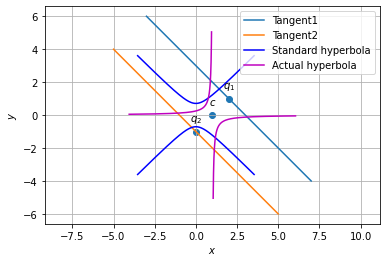
\includegraphics[width=\columnwidth]{./solutions/1/14/graph7.png}
	\caption{The standard and actual hyperbola.}
\end{figure}

    \item Solve $\frac{3x-4}{2} \geq \frac{x+1}{4}-1$. Show the graph of the solutions on number line.
\\
\solution 
The given curve 
\begin{align}
	y =\frac{1}{x-1}
\end{align}
can be expressed as 
\begin{align}
	xy - y - 1 = 0 \label{eq:solutions/1/14/eq:hyperbola}
\end{align}
Hence, we have
\begin{align}
	\vec{V} = \frac{1}{2}\myvec{0 & 1 \\ 1 & 0}, 
	\vec{u} = \frac{1}{2}\myvec{0 \\-1},
	f = -1
\end{align}
Since $\mydet{\vec{V}} < 0$, the equation \eqref{eq:solutions/1/14/eq:hyperbola} represents hyperbola.
To find the values of $\lambda_1$ and $\lambda_2$, consider the characteristic equation,
\begin{align}
	\mydet{\lambda\vec{I} - \vec{V}} &= 0\\
	\implies \mydet{\myvec{\lambda & 0\\0 & \lambda} - \myvec{0 & \frac{1}{2} \\ \frac{1}{2} & 0}} &= 0\\
	\implies \mydet{ \lambda & \frac{-1}{2} \\ \frac{-1}{2} & \lambda} &= 0\\
	\implies \lambda_1 &= \frac{1}{2} , \lambda_2 = \frac{-1}{2}
\end{align}
In addition, given the slope -1, the direction and normal vectors are given by 
\begin{align}
	\vec{m} = \myvec{1 \\ -1} \\
	\vec{n} = \myvec{ 1 \\ 1}
\end{align}
The parameters of hyperbola are as follows:
\begin{align}
	\vec{c} &= -\vec{V}^{-1}\vec{u} \\
	&= -\myvec{0 & 2\\ 2 & 0}\myvec{0 \\ -\frac{1}{2}} \\
	&= \myvec{1 \\ 0}\\
	axes &= \begin{cases}
	\sqrt{\frac{\vec{u}^T\vec{V}^{-1}\vec{u} - f}{\lambda_1}} = \sqrt{2}\\
 \sqrt{\frac{f-\vec{u}^T\vec{V}^{-1}\vec{u}}{\lambda_2}} = \sqrt{2}
\end{cases}
\end{align}
which represents the standard hyperbola equation,
\begin{align}
	\frac{x^2}{2} - \frac{x^2}{2} = 1
\end{align}
The points of contact are given by 
\begin{align}
  \tiny{K} &=\pm \sqrt{\frac{\vec{u}^T\vec{V}^{-1}\vec{u} - f}{\vec{n}^T\vec{V}^{-1}\vec{n}}}
  = \pm \frac{1}{2}\\
  \vec{q} &= \vec{V}^{-1}(k\vec{n}-\vec{u})\\
  \vec{q_1} &= \myvec{0 & 2\\2 & 0} \sbrak{\frac{1}{2}\myvec{1 \\ 1} - \myvec{0\\ \frac{-1}{2}}}\\
  &= \myvec{2 \\ 1}\\
  \vec{q_2} &= \myvec{0 & 2\\2 & 0} \sbrak{\frac{-1}{2}\myvec{1 \\ 1} - \myvec{0\\ \frac{-1}{2}}}\\
  &= \myvec{0 \\ -1}
\end{align} 
$\therefore$ The tangents are given by
\begin{align}
	\myvec{1 & 1} \brak{\vec{x} - \myvec{2 \\ 1}} = 0 \\
	\myvec{1 & 1} \brak{\vec{x} - \myvec{0 \\ -1}} = 0
\end{align}
The desired equations of all lines having slope -1 that are tangents to the curve $\frac{1}{x-1}, x \neq 1$ are given by
\begin{align}
	\myvec{1 & 1}\vec{x} &= 3 \\
	\myvec{1 & 1}\vec{x} &= -1 
\end{align}
The above results are verified in the following figure.
\begin{figure}[h!] \label{eq:solutions/1/14/fig:tangents}
	\centering
	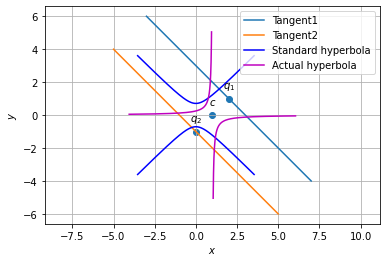
\includegraphics[width=\columnwidth]{./solutions/1/14/graph7.png}
	\caption{The standard and actual hyperbola.}
\end{figure}

    \item The marks obtained by a student of Class XI in first and second terminal examination are 62 and 48, respectively. Find the minimum marks he should get in the annual examination to have an average of at least 60 marks.
\\
\solution 
The given curve 
\begin{align}
	y =\frac{1}{x-1}
\end{align}
can be expressed as 
\begin{align}
	xy - y - 1 = 0 \label{eq:solutions/1/14/eq:hyperbola}
\end{align}
Hence, we have
\begin{align}
	\vec{V} = \frac{1}{2}\myvec{0 & 1 \\ 1 & 0}, 
	\vec{u} = \frac{1}{2}\myvec{0 \\-1},
	f = -1
\end{align}
Since $\mydet{\vec{V}} < 0$, the equation \eqref{eq:solutions/1/14/eq:hyperbola} represents hyperbola.
To find the values of $\lambda_1$ and $\lambda_2$, consider the characteristic equation,
\begin{align}
	\mydet{\lambda\vec{I} - \vec{V}} &= 0\\
	\implies \mydet{\myvec{\lambda & 0\\0 & \lambda} - \myvec{0 & \frac{1}{2} \\ \frac{1}{2} & 0}} &= 0\\
	\implies \mydet{ \lambda & \frac{-1}{2} \\ \frac{-1}{2} & \lambda} &= 0\\
	\implies \lambda_1 &= \frac{1}{2} , \lambda_2 = \frac{-1}{2}
\end{align}
In addition, given the slope -1, the direction and normal vectors are given by 
\begin{align}
	\vec{m} = \myvec{1 \\ -1} \\
	\vec{n} = \myvec{ 1 \\ 1}
\end{align}
The parameters of hyperbola are as follows:
\begin{align}
	\vec{c} &= -\vec{V}^{-1}\vec{u} \\
	&= -\myvec{0 & 2\\ 2 & 0}\myvec{0 \\ -\frac{1}{2}} \\
	&= \myvec{1 \\ 0}\\
	axes &= \begin{cases}
	\sqrt{\frac{\vec{u}^T\vec{V}^{-1}\vec{u} - f}{\lambda_1}} = \sqrt{2}\\
 \sqrt{\frac{f-\vec{u}^T\vec{V}^{-1}\vec{u}}{\lambda_2}} = \sqrt{2}
\end{cases}
\end{align}
which represents the standard hyperbola equation,
\begin{align}
	\frac{x^2}{2} - \frac{x^2}{2} = 1
\end{align}
The points of contact are given by 
\begin{align}
  \tiny{K} &=\pm \sqrt{\frac{\vec{u}^T\vec{V}^{-1}\vec{u} - f}{\vec{n}^T\vec{V}^{-1}\vec{n}}}
  = \pm \frac{1}{2}\\
  \vec{q} &= \vec{V}^{-1}(k\vec{n}-\vec{u})\\
  \vec{q_1} &= \myvec{0 & 2\\2 & 0} \sbrak{\frac{1}{2}\myvec{1 \\ 1} - \myvec{0\\ \frac{-1}{2}}}\\
  &= \myvec{2 \\ 1}\\
  \vec{q_2} &= \myvec{0 & 2\\2 & 0} \sbrak{\frac{-1}{2}\myvec{1 \\ 1} - \myvec{0\\ \frac{-1}{2}}}\\
  &= \myvec{0 \\ -1}
\end{align} 
$\therefore$ The tangents are given by
\begin{align}
	\myvec{1 & 1} \brak{\vec{x} - \myvec{2 \\ 1}} = 0 \\
	\myvec{1 & 1} \brak{\vec{x} - \myvec{0 \\ -1}} = 0
\end{align}
The desired equations of all lines having slope -1 that are tangents to the curve $\frac{1}{x-1}, x \neq 1$ are given by
\begin{align}
	\myvec{1 & 1}\vec{x} &= 3 \\
	\myvec{1 & 1}\vec{x} &= -1 
\end{align}
The above results are verified in the following figure.
\begin{figure}[h!] \label{eq:solutions/1/14/fig:tangents}
	\centering
	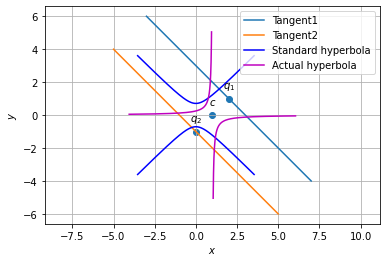
\includegraphics[width=\columnwidth]{./solutions/1/14/graph7.png}
	\caption{The standard and actual hyperbola.}
\end{figure}

    \item Find all pairs of consecutive odd natural numbers, both of which are larger than 10, such that their sum is less than 40.
\\
\solution 
	
Let x be an odd natural number and y be the odd natural number consecutive to x.
	\begin{align}
	\therefore y=x+2
	\end{align}
	We need to find x and y  such that 
	\begin{multline}
x,y >10 \text{ and } x+y<40\\
\therefore x+x+2<40\\
2x+2<40\\
x+1<20\\
x<19
	\end{multline}
	
	
	Hence the condition is satisfied when $x>10$ and $x<19$
	
	
	
	The following python code computes the required pairs of consecutive odd natural numbers which satisfy the required condition, shown in Fig.\ref{fig:3.11.5_fifteen}.
	\begin{lstlisting}
	./solutions/5/codes/lines/q15.py
	\end{lstlisting}
	\begin{figure}[!ht]
	\centering
	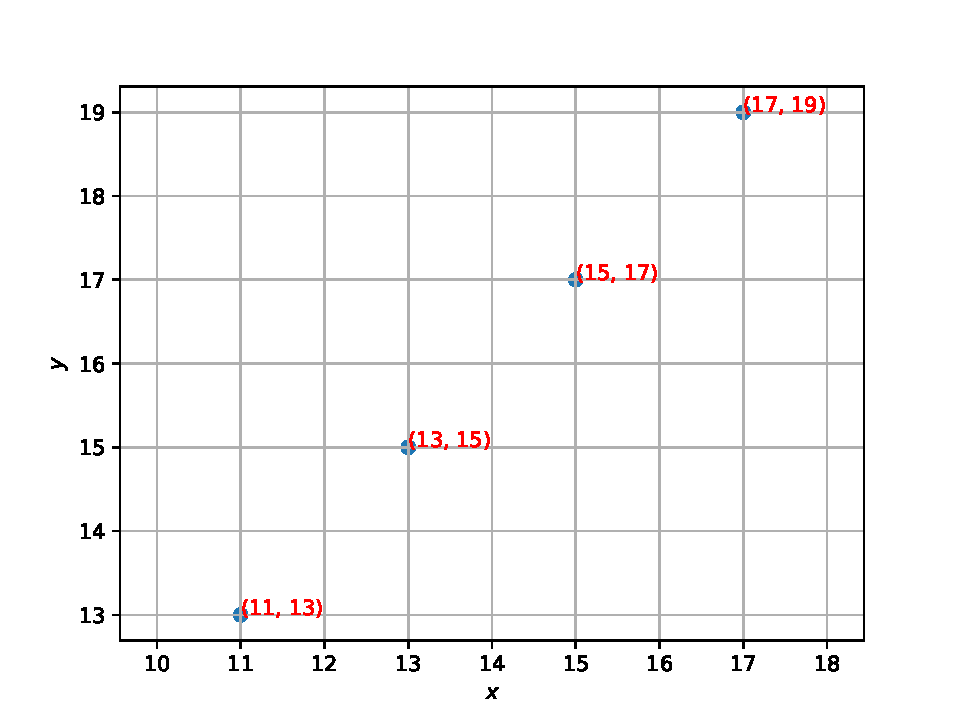
\includegraphics[width=\columnwidth]{./solutions/5/figs/lines/q15.eps}
	\caption{}
	\label{fig:3.11.5_fifteen}	
	\end{figure}

    \item Solve 3x+2y $>$ 6 graphically.
\\
\solution 
The given curve 
\begin{align}
	y =\frac{1}{x-1}
\end{align}
can be expressed as 
\begin{align}
	xy - y - 1 = 0 \label{eq:solutions/1/14/eq:hyperbola}
\end{align}
Hence, we have
\begin{align}
	\vec{V} = \frac{1}{2}\myvec{0 & 1 \\ 1 & 0}, 
	\vec{u} = \frac{1}{2}\myvec{0 \\-1},
	f = -1
\end{align}
Since $\mydet{\vec{V}} < 0$, the equation \eqref{eq:solutions/1/14/eq:hyperbola} represents hyperbola.
To find the values of $\lambda_1$ and $\lambda_2$, consider the characteristic equation,
\begin{align}
	\mydet{\lambda\vec{I} - \vec{V}} &= 0\\
	\implies \mydet{\myvec{\lambda & 0\\0 & \lambda} - \myvec{0 & \frac{1}{2} \\ \frac{1}{2} & 0}} &= 0\\
	\implies \mydet{ \lambda & \frac{-1}{2} \\ \frac{-1}{2} & \lambda} &= 0\\
	\implies \lambda_1 &= \frac{1}{2} , \lambda_2 = \frac{-1}{2}
\end{align}
In addition, given the slope -1, the direction and normal vectors are given by 
\begin{align}
	\vec{m} = \myvec{1 \\ -1} \\
	\vec{n} = \myvec{ 1 \\ 1}
\end{align}
The parameters of hyperbola are as follows:
\begin{align}
	\vec{c} &= -\vec{V}^{-1}\vec{u} \\
	&= -\myvec{0 & 2\\ 2 & 0}\myvec{0 \\ -\frac{1}{2}} \\
	&= \myvec{1 \\ 0}\\
	axes &= \begin{cases}
	\sqrt{\frac{\vec{u}^T\vec{V}^{-1}\vec{u} - f}{\lambda_1}} = \sqrt{2}\\
 \sqrt{\frac{f-\vec{u}^T\vec{V}^{-1}\vec{u}}{\lambda_2}} = \sqrt{2}
\end{cases}
\end{align}
which represents the standard hyperbola equation,
\begin{align}
	\frac{x^2}{2} - \frac{x^2}{2} = 1
\end{align}
The points of contact are given by 
\begin{align}
  \tiny{K} &=\pm \sqrt{\frac{\vec{u}^T\vec{V}^{-1}\vec{u} - f}{\vec{n}^T\vec{V}^{-1}\vec{n}}}
  = \pm \frac{1}{2}\\
  \vec{q} &= \vec{V}^{-1}(k\vec{n}-\vec{u})\\
  \vec{q_1} &= \myvec{0 & 2\\2 & 0} \sbrak{\frac{1}{2}\myvec{1 \\ 1} - \myvec{0\\ \frac{-1}{2}}}\\
  &= \myvec{2 \\ 1}\\
  \vec{q_2} &= \myvec{0 & 2\\2 & 0} \sbrak{\frac{-1}{2}\myvec{1 \\ 1} - \myvec{0\\ \frac{-1}{2}}}\\
  &= \myvec{0 \\ -1}
\end{align} 
$\therefore$ The tangents are given by
\begin{align}
	\myvec{1 & 1} \brak{\vec{x} - \myvec{2 \\ 1}} = 0 \\
	\myvec{1 & 1} \brak{\vec{x} - \myvec{0 \\ -1}} = 0
\end{align}
The desired equations of all lines having slope -1 that are tangents to the curve $\frac{1}{x-1}, x \neq 1$ are given by
\begin{align}
	\myvec{1 & 1}\vec{x} &= 3 \\
	\myvec{1 & 1}\vec{x} &= -1 
\end{align}
The above results are verified in the following figure.
\begin{figure}[h!] \label{eq:solutions/1/14/fig:tangents}
	\centering
	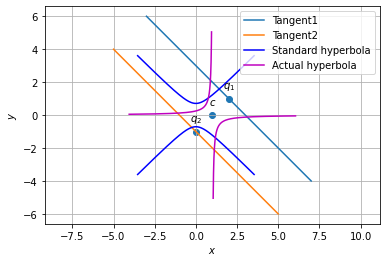
\includegraphics[width=\columnwidth]{./solutions/1/14/graph7.png}
	\caption{The standard and actual hyperbola.}
\end{figure}

    \item Solve 3x-6 $\geq$ 0 graphically in a two dimensional plane.
\\
\solution 
The given curve 
\begin{align}
	y =\frac{1}{x-1}
\end{align}
can be expressed as 
\begin{align}
	xy - y - 1 = 0 \label{eq:solutions/1/14/eq:hyperbola}
\end{align}
Hence, we have
\begin{align}
	\vec{V} = \frac{1}{2}\myvec{0 & 1 \\ 1 & 0}, 
	\vec{u} = \frac{1}{2}\myvec{0 \\-1},
	f = -1
\end{align}
Since $\mydet{\vec{V}} < 0$, the equation \eqref{eq:solutions/1/14/eq:hyperbola} represents hyperbola.
To find the values of $\lambda_1$ and $\lambda_2$, consider the characteristic equation,
\begin{align}
	\mydet{\lambda\vec{I} - \vec{V}} &= 0\\
	\implies \mydet{\myvec{\lambda & 0\\0 & \lambda} - \myvec{0 & \frac{1}{2} \\ \frac{1}{2} & 0}} &= 0\\
	\implies \mydet{ \lambda & \frac{-1}{2} \\ \frac{-1}{2} & \lambda} &= 0\\
	\implies \lambda_1 &= \frac{1}{2} , \lambda_2 = \frac{-1}{2}
\end{align}
In addition, given the slope -1, the direction and normal vectors are given by 
\begin{align}
	\vec{m} = \myvec{1 \\ -1} \\
	\vec{n} = \myvec{ 1 \\ 1}
\end{align}
The parameters of hyperbola are as follows:
\begin{align}
	\vec{c} &= -\vec{V}^{-1}\vec{u} \\
	&= -\myvec{0 & 2\\ 2 & 0}\myvec{0 \\ -\frac{1}{2}} \\
	&= \myvec{1 \\ 0}\\
	axes &= \begin{cases}
	\sqrt{\frac{\vec{u}^T\vec{V}^{-1}\vec{u} - f}{\lambda_1}} = \sqrt{2}\\
 \sqrt{\frac{f-\vec{u}^T\vec{V}^{-1}\vec{u}}{\lambda_2}} = \sqrt{2}
\end{cases}
\end{align}
which represents the standard hyperbola equation,
\begin{align}
	\frac{x^2}{2} - \frac{x^2}{2} = 1
\end{align}
The points of contact are given by 
\begin{align}
  \tiny{K} &=\pm \sqrt{\frac{\vec{u}^T\vec{V}^{-1}\vec{u} - f}{\vec{n}^T\vec{V}^{-1}\vec{n}}}
  = \pm \frac{1}{2}\\
  \vec{q} &= \vec{V}^{-1}(k\vec{n}-\vec{u})\\
  \vec{q_1} &= \myvec{0 & 2\\2 & 0} \sbrak{\frac{1}{2}\myvec{1 \\ 1} - \myvec{0\\ \frac{-1}{2}}}\\
  &= \myvec{2 \\ 1}\\
  \vec{q_2} &= \myvec{0 & 2\\2 & 0} \sbrak{\frac{-1}{2}\myvec{1 \\ 1} - \myvec{0\\ \frac{-1}{2}}}\\
  &= \myvec{0 \\ -1}
\end{align} 
$\therefore$ The tangents are given by
\begin{align}
	\myvec{1 & 1} \brak{\vec{x} - \myvec{2 \\ 1}} = 0 \\
	\myvec{1 & 1} \brak{\vec{x} - \myvec{0 \\ -1}} = 0
\end{align}
The desired equations of all lines having slope -1 that are tangents to the curve $\frac{1}{x-1}, x \neq 1$ are given by
\begin{align}
	\myvec{1 & 1}\vec{x} &= 3 \\
	\myvec{1 & 1}\vec{x} &= -1 
\end{align}
The above results are verified in the following figure.
\begin{figure}[h!] \label{eq:solutions/1/14/fig:tangents}
	\centering
	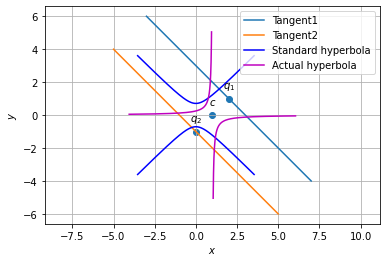
\includegraphics[width=\columnwidth]{./solutions/1/14/graph7.png}
	\caption{The standard and actual hyperbola.}
\end{figure}
    
\item 2x+y $\geq$ 6, 3x+4y $\leq$ 12.
    \\
    \solution
    
\documentclass[journal,12pt,twocolumn]{IEEEtran}
\title{
3 to 8 Decoder through VAMAN FPGA
}
\author{Kukunuri Sampath Govardhan}
\begin{document}
\maketitle
\tableofcontents
\begin{abstract}
This document shows how to use VAMAN Board as a 3 to 8 Decoder in FPGA
\end{abstract}
\section{Components}
\begin{table}[h]
    \centering
    \begin{tabular}{| c | c | c |}
       \hline
       \textbf{Component}  &  \textbf{Value}  &  \textbf{Qunatity}\\
       \hline
         Resistor  &  220Ohm  &  8  \\
         \hline
         LED  &  Red  &  8  \\
         \hline
         VAMAN Board  &  & 1  \\
         \hline
         Jumper Wires  &  M-F  &  20  \\
         \hline
         BreadBoard  &    &  1\\
         \hline
         
    \end{tabular}
    \caption{}
    \label{tab:my_label}
\end{table}
\section{Setup}
\textbf{Problem 2.1} Make connections between the Vaman Board(PYGMY) and LED's as shown in Table 2 \\

\textbf{Problem 2.2} Connect anodes of LED's to the pins using resistors and cathodes to ground(gnd).\\
\begin{table}[h]
    \centering
    \begin{tabular}{| c | c | c | c | c | c | c | c |}
        \hline
         IO\_4 & IO\_5 & IO\_6 & IO\_7 & IO\_8 & IO\_10 & IO\_11 & IO\_12  \\
       \hline
       led1 & led2 & led3 & led4 & led5 & led6 & led7 & led8  \\
         \hline
    \end{tabular}
    \caption{}
    \label{tab:my_label}
\end{table}
\\
\textbf{Problem 2.3} Connect the input pins X, Y, Z to Vaman as shown in Table 3.\\

    \begin{table}[h]
    \centering
    \begin{tabular}{| c | c | c |}
    \hline
    \textbf{X} & \textbf{Y} & \textbf{Z} \\
    \hline
    IO\_23 & IO\_28 & IO\_31  \\
    \hline
    \end{tabular}
    \caption{}
    \label{tab:my_label}
 \end{table}


\section{Software}
\textbf{Problem 3.1} Execute the following script in termux which compiles the code and sends it to pi. \\
\vspace{1cm}
\begin{table}[h]
    \centering
    \begin{tabular}{| c |}
    \hline
    wget https://github.com/mygit-sampath-govardhan/fwc-iith-assignments\\/blob/14bf619b0f2efd421bb36bb4357cc751132bf78b/Assignment-9\\(ARM-3to8\%20decoder)/script.sh\\
    \hline
    \end{tabular}
\end{table}
\textbf{Note:} Change the ipaddress accordingly.\\
\\
\textbf{Problem 3.2} Now execute the following script in pi which flashes .bin file to Vaman board, and verify all the outputs as mentioned in Truth table (Table 4) by modifying the inputs X, Y, Z to 0's and 1's respectively. \\
\begin{table}[h]
    \centering
    \begin{tabular}{| c |}
    \hline
    wget https://github.com/mygit-sampath-govardhan/fwc-iith-assignments\\/blob/14bf619b0f2efd421bb36bb4357cc751132bf78b/Assignment-9\\(ARM-3to8\%20decoder)/In\%20pi/arm.sh\\
    \hline
    \end{tabular}
\end{table}

\textbf{Note:} Output pins IO\_4-8,IO\_10-12 are referenced as A-H respectively and input pins IO\_23,28,31 are referred as X,Y,Z respectively.\\

    \begin{table}[h]
    \centering
    \begin{tabular}{| c | c | c || c | c | c | c | c | c | c | c |}
    \hline
    \textbf{X} & \textbf{Y} & \textbf{Z} & \textbf{A} & \textbf{B} & \textbf{C} & \textbf{D} & \textbf{E} & \textbf{F} & \textbf{G} & \textbf{H} \\
    \hline
    0 & 0 & 0 & 0 & 0 & 0 & 0 & 0 & 0 & 0 & 1  \\
    \hline
    0 & 0 & 1 & 0 & 0 & 0 & 0 & 0 & 0 & 1 & 0  \\
    \hline
    0 & 1 & 0 & 0 & 0 & 0 & 0 & 0 & 1 & 0 & 0  \\
    \hline
    0 & 1 & 1 & 0 & 0 & 0 & 0 & 1 & 0 & 0 & 0  \\
    \hline
    1 & 0 & 0 & 0 & 0 & 0 & 1 & 0 & 0 & 0 & 0  \\
    \hline
    1 & 0 & 1 & 0 & 0 & 1 & 0 & 0 & 0 & 0 & 0  \\
    \hline
    1 & 1 & 0 & 0 & 1 & 0 & 0 & 0 & 0 & 0 & 0  \\
    \hline
    1 & 1 & 1 & 1 & 0 & 0 & 0 & 0 & 0 & 0 & 0  \\
    \hline
    \end{tabular}
    \caption{Truth Table}
    \label{tab:my_label}
 \end{table}
\section{Solution}

In the Truth table (Table3) X,Y,Z are inputs and A,B,C,D,E,F,G,H are outputs. This table represents the system that behaves as a 3 to 8 decoder. Using Boolean logic, \\
 \begin{center}
     A= X' Y' Z'\\
 \end{center}
  \begin{center}
      B= X' Y' Z\\
 \end{center}
  \begin{center}
      C= X' Y Z'\\
 \end{center}
  \begin{center}
      D= X' Y Z\\
 \end{center}
  \begin{center}
     E= X Y' Z'\\
 \end{center}
  \begin{center}
     F= X Y' Z\\
 \end{center}
  \begin{center}
     G= X Y Z'\\
 \end{center}
  \begin{center}
     H= X Y Z\\
 \end{center} 
 \section{Conclusion}
 A 3 to 8 decoder has 3 inputs and 8 outputs are generated using these 3 inputs.\\
 \\
  Here 3 to 8 decoder with Vaman Board has been successfully verified.\\
\end{document}


    \item 2x-y $>$ 1, x-2y $<$ -1.
    \\
    \solution
    
%
Let
\begin{align}
\label{eq:1}
\begin{split}
2x-y &> 1,
\\-x+2y &> 1.
\end{split}
\end{align}
\\
Let $u_1 > 0, u_2 > 0$. This may be expressed as
\begin{align}
\vec{u} = \myvec{u_1\\u_2} &> \vec{0}
\end{align}
Now we have,
\begin{align}
\myvec{2&-1 \\ -1&2 }\vec{x} &> \myvec{1 \\ 1}   
\\
\myvec{2&-1 \\ -1&2 }\vec{x}-\vec{u} &= \myvec{1 \\ 1} 
\\
\text{or, } \myvec{2&-1 \\ -1&2 }\vec{x} &= \myvec{1 \\ 1}  + \vec{u}
\end{align}
Resulting in
\begin{align}
\vec{x} &= \myvec{2 & -1 \\ -1 & 2}^{-1}\myvec{1 \\ 1} +\myvec{2 & -1 \\ -1 & 2}^{-1} \vec{u}
\\
\vec{x }&=\myvec{1 \\ 1} +\frac{1}{3}\myvec{2 & 1 \\ 1 & 2}\vec{u}
\end{align} 
Thus , the solution of the system of inequalities can be determined graphically and the desired region is the shaded triangle which is represented in Fig. \ref{fig: Graphical Solution}
\begin{figure}[!ht]
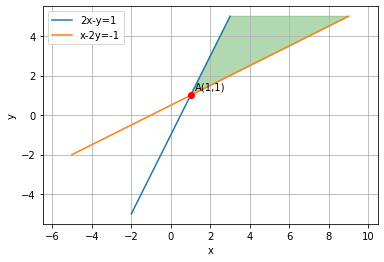
\includegraphics[width=\columnwidth]{solutions/su2021/2/50/Graphical Solution.png}
\caption{Graphical Solution}
\label{fig: Graphical Solution}
\end{figure}



    From the given information, for 
\begin{align}
\Vec{A} &=  \myvec{2 \\ 5 } , \Vec{B} =  \myvec{-3 \\ 6},
\vec{m} &= \vec{A}-\vec{B}
\\
& = \myvec{5 \\ -1}
\\
\implies \vec{n}& = \myvec{5 \\ -1}
\end{align}
Let 
\begin{align}
    \vec{P} = \myvec{-3\\5}
\end{align}
The equation of the desired line is then obtained as
\begin{align}
\label{linform/15/eq:line_norm_vec}
\vec{n}^T\brak{\vec{x}-\vec{P}} &= 0
\\
\implies \myvec{5 & -1} \vec{x} &= -20
\end{align}
and plotted in Fig. \ref{linform/15/fig: Perpendicular Bisector}	
\begin{figure}[!ht]
\centering
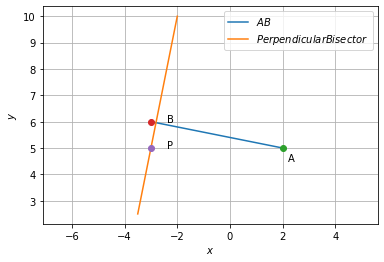
\includegraphics[width=\columnwidth]{solutions/su2021/2/15/download (6).png}
\caption{Perpendicular Bisector}
\label{linform/15/fig: Perpendicular Bisector}	
\end{figure}

    \item 2x+y $\geq$ 8, x+2y $\geq$ 10.
    \\
    \solution
    From the given information, for 
\begin{align}
\Vec{A} &=  \myvec{2 \\ 5 } , \Vec{B} =  \myvec{-3 \\ 6},
\vec{m} &= \vec{A}-\vec{B}
\\
& = \myvec{5 \\ -1}
\\
\implies \vec{n}& = \myvec{5 \\ -1}
\end{align}
Let 
\begin{align}
    \vec{P} = \myvec{-3\\5}
\end{align}
The equation of the desired line is then obtained as
\begin{align}
\label{linform/15/eq:line_norm_vec}
\vec{n}^T\brak{\vec{x}-\vec{P}} &= 0
\\
\implies \myvec{5 & -1} \vec{x} &= -20
\end{align}
and plotted in Fig. \ref{linform/15/fig: Perpendicular Bisector}	
\begin{figure}[!ht]
\centering
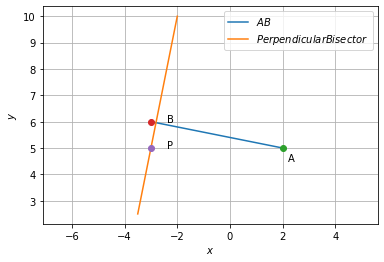
\includegraphics[width=\columnwidth]{solutions/su2021/2/15/download (6).png}
\caption{Perpendicular Bisector}
\label{linform/15/fig: Perpendicular Bisector}	
\end{figure}

    \item 3x+4y $\leq$ 60, x+3y $\leq$ 30, x $\geq$ 0, y $\geq$ 0.
    \\
    \solution
    
From the given inequalities we have,
\begin{align}
    \myvec{-3&-4 \\ -1&-3 \\ 1&0 \\ 0&1}\vec{x} \succeq \myvec{-60 \\ -30 \\ 0 \\ 0}
\end{align}
Which can be further written as
\begin{align}
   \myvec{-3&-4 \\ -1&-3 }\vec{x} \succeq \myvec{-60 \\ -30} 
\end{align}
Let $u_1 \ge 0, u_2 \ge 0$.  This may be expressed as
\begin{align}
\vec{u} = \myvec{u_1\\u_2}\succeq \vec{0}
\end{align}
Now we have,
\begin{align}
  \myvec{-3&-4 \\ -1&-3 }\vec{x} \succeq \myvec{-60 \\ -30}  + \vec{u} 
\end{align}
\begin{align}
        \vec{x} = \myvec{-3 & -4 \\ -1 & -3}^{-1}\myvec{-60 \\ -30} + \myvec{-3 & -4 \\ -1 & -3}^{-1}\vec{u}
        \\
        \implies \vec{x} = \frac{1}{5}\myvec{60 \\ 30}+\frac{1}{5}\myvec{-3&4 \\ 1&-3}\vec{u}
        \\
        \vec{x}=\myvec{12 \\ 6}+\frac{1}{5}\myvec{-3&4 \\ 1&-3}\vec{u}
    \end{align}
Thus the solution of the system of inequalities can be determined graphically, which is represented in Fig.     \ref{ineq/2/55/Graphical solution}.
%
\begin{figure}[ht]
    \centering
    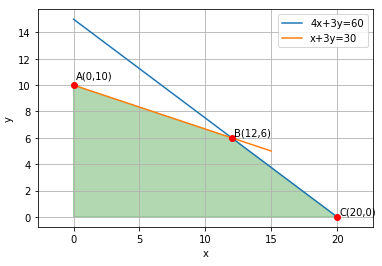
\includegraphics[width=\columnwidth]{solutions/su2021/2/55/Graphical solution region.PNG}
    \caption{Graphical solution}
    \label{ineq/2/55/Graphical solution}
\end{figure}






    \item x-2y $\leq$ 3, 3x+4y $\geq$ 12, x $\geq$ 0, y $\geq$ 1.
    \\
    \solution
    \begin{enumerate}[label=\alph*.]
    \item  Given $\triangle ABC$ with vertices
    \begin{align}
      \vec{A} = \myvec{4 \\ 2}, \vec{B}=\myvec{6 \\ 5},         \vec{C}=\myvec{1 \\ 4}  
    \end{align}
    Given that the median from $\vec{A}$ meets $BC$ at $\vec{D}$, now the coordinate of $\vec{D}$ is given as,
    \begin{align}
        \vec{D} = \frac{\vec{B}+\vec{C}}{2} = \frac{\myvec{6 \\ 5}+\myvec{1 \\ 4}}{2}\\
        \implies \vec{D} = \myvec{\frac{7}{2} \\ \frac{9}{2}}
    \end{align}
    \item  Result :The coordinates of point $\vec{C}$ dividing the line $AB$ in the ratio $m:n$ is given by 
    \begin{align}
      \frac{n\vec{A}+m\vec{B}}{m+n}  \label{vectors/2/eq:1}
    \end{align}
    Given that the point $\vec{P}$ divides $AD$ in the ratio $2:1$, now to find $\vec{P}$ we use \eqref{vectors/2/eq:1},
    \begin{align}
        \vec{P}=\frac{1\myvec{4\\2}+2\myvec{\frac{7}{2}\\ \frac{9}{2}}}{3}=\myvec{\frac{11}{3} \\ \frac{11}{3}}
    \end{align}
    \item Given that the point $\vec{Q}$ on the median $BE$ divides it in the ratio $2:1$, first we find $\vec{E}$,
    \begin{align}
        \vec{E} =\frac{\vec{A}+\vec{C}}{2} = \frac{\myvec{4 \\ 2}+\myvec{1 \\ 4}}{2}\\
        \implies \vec{E} = \myvec{\frac{5}{2} \\ 3}.
    \end{align}
    Now we find $\vec{Q}$ using \eqref{vectors/2/eq:1}
    \begin{align}
       \vec{Q}=\frac{1\myvec{6\\5}+2\myvec{\frac{5}{2}\\3}}{3}=\myvec{\frac{11}{3} \\ \frac{11}{3}} 
    \end{align}
    Similarly,Given that the point $\vec{R}$ on the median $CF$ divides it in the ratio $2:1$, first we find $\vec{F}$,
    \begin{align}
        \vec{F} =\frac{\vec{A}+\vec{B}}{2} = \frac{\myvec{4 \\ 2}+\myvec{6 \\ 5}}{2}\\
        \implies \vec{F} = \myvec{5 \\ \frac{7}{2}}.
    \end{align}
    Now we find $\vec{R}$ using \eqref{vectors/2/eq:1}
    \begin{align}
       \vec{R}=\frac{1\myvec{1\\4}+2\myvec{5 \\ \frac{7}{2}}}{3}=\myvec{\frac{11}{3} \\ \frac{11}{3}} 
    \end{align}
    \end{enumerate}
    The plot of the $\triangle ABC$ is given in Fig.     \ref{vectors/2/fig:triangle ABC}.
    %
    \begin{figure}[ht]
        \centering
        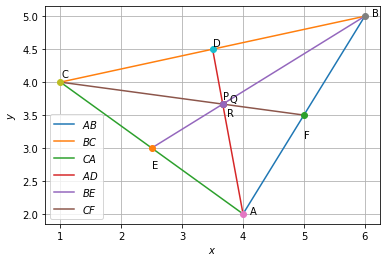
\includegraphics[width=\columnwidth]{solutions/su2021/2/2/TriangleABC.PNG}
        \caption{Plot of $\triangle ABC$}
        \label{vectors/2/fig:triangle ABC}
    \end{figure}
    \item 4x+3y $\leq$ 60, y $\geq$ 2x, x $\geq$ 3, x,y $\geq$ 0.
    \\
    \solution
    
\documentclass[journal,12pt,twocolumn]{IEEEtran}
\title{
3 to 8 Decoder through VAMAN ESP-32
}
\author{Kukunuri Sampath Govardhan}
\begin{document}
\maketitle
\tableofcontents
\section{Components}
\begin{table}[h]
    \centering
    \begin{tabular}{| c | c | c |}
       \hline
       \textbf{Component}  &  \textbf{Value}  &  \textbf{Qunatity}\\
       \hline
         Resistor  &  220Ohm  &  8  \\
         \hline
         LED  &  Red  &  8  \\
         \hline
         VAMAN Board  &  & 1  \\
         \hline
         Jumper Wires  &  M-F  &  20  \\
         \hline
         BreadBoard  &    &  1\\
         \hline
         
    \end{tabular}
    \caption{}
    \label{tab:my_label}
\end{table}
\section{Setup}
\textbf{Problem 2.1} Make connections between the Vaman Board(ESP-32) and LED's as shown in Table 2 \\

\textbf{Problem 2.2} Connect anodes of LED's to the pins using resistors and cathodes to ground(gnd).\\
\begin{table}[h]
    \centering
    \begin{tabular}{| c | c | c | c | c | c | c | c |}
        \hline
         IO\_11 & IO\_12 & IO\_13 & IO\_14 & IO\_15 & IO\_16 & IO\_17 & IO\_18    \\
       \hline
       led1 & led2 & led3 & led4 & led5 & led6 & led7 & led8  \\
         \hline
    \end{tabular}
    \caption{}
    \label{tab:my_label}
\end{table}
\\
\textbf{Problem 2.3} Connect the input pins X, Y, Z to Vaman as shown in Table 3.\\

    \begin{table}[h]
    \centering
    \begin{tabular}{| c | c | c |}
    \hline
    \textbf{X} & \textbf{Y} & \textbf{Z} \\
    \hline
    IO\_8 & IO\_9 & IO\_10  \\
    \hline
    \end{tabular}
    \caption{}
    \label{tab:my_label}
 \end{table}


\section{Software}
\textbf{Problem 3.1} Execute the following script in termux which compiles the code and generates a .bin file and sends it to Vaman board. \\
\vspace{1cm}
\begin{table}[h]
    \centering
    \begin{tabular}{| c |}
    \hline
wget https://github.com/mygit-sampath-govardhan\\/fwc-iith-assignments/blob/98ed8708b8864dc568f557e7fcead70f441b7449\\/Assignment-11(ESP\_32\%20-\%203\%20to\%208\%20decoder)/script.sh\\
    \hline
    \end{tabular}
\end{table}
\textbf{Note:} Change the ipaddress accordingly.\\
\\
\textbf{Problem 3.2} Verify all the outputs as mentioned in Truth table (Table 4) by modifying the inputs X, Y, Z to 0's and 1's respectively. \\

\textbf{Note:} Output pins IO\_11-18 are referenced as A-H respectively and input pins IO\_8,9,10 are referred as X,Y,Z respectively.\\

    \begin{table}[h]
    \centering
    \begin{tabular}{| c | c | c || c | c | c | c | c | c | c | c |}
    \hline
    \textbf{X} & \textbf{Y} & \textbf{Z} & \textbf{A} & \textbf{B} & \textbf{C} & \textbf{D} & \textbf{E} & \textbf{F} & \textbf{G} & \textbf{H} \\
    \hline
    0 & 0 & 0 & 0 & 0 & 0 & 0 & 0 & 0 & 0 & 1  \\
    \hline
    0 & 0 & 1 & 0 & 0 & 0 & 0 & 0 & 0 & 1 & 0  \\
    \hline
    0 & 1 & 0 & 0 & 0 & 0 & 0 & 0 & 1 & 0 & 0  \\
    \hline
    0 & 1 & 1 & 0 & 0 & 0 & 0 & 1 & 0 & 0 & 0  \\
    \hline
    1 & 0 & 0 & 0 & 0 & 0 & 1 & 0 & 0 & 0 & 0  \\
    \hline
    1 & 0 & 1 & 0 & 0 & 1 & 0 & 0 & 0 & 0 & 0  \\
    \hline
    1 & 1 & 0 & 0 & 1 & 0 & 0 & 0 & 0 & 0 & 0  \\
    \hline
    1 & 1 & 1 & 1 & 0 & 0 & 0 & 0 & 0 & 0 & 0  \\
    \hline
    \end{tabular}
    \caption{Truth Table}
    \label{tab:my_label}
 \end{table}
\section{Solution}

In the Truth table (Table3) X,Y,Z are inputs and A,B,C,D,E,F,G,H are outputs. This table represents the system that behaves as a 3 to 8 decoder. Using Boolean logic, \\
 \begin{center}
     A= X' Y' Z'\\
 \end{center}
  \begin{center}
      B= X' Y' Z\\
 \end{center}
  \begin{center}
      C= X' Y Z'\\
 \end{center}
  \begin{center}
      D= X' Y Z\\
 \end{center}
  \begin{center}
     E= X Y' Z'\\
 \end{center}
  \begin{center}
     F= X Y' Z\\
 \end{center}
  \begin{center}
     G= X Y Z'\\
 \end{center}
  \begin{center}
     H= X Y Z\\
 \end{center} 
 \section{Conclusion}
 A 3 to 8 decoder has 3 inputs and 8 outputs are generated using these 3 inputs.\\
 \\
  Here 3 to 8 decoder with Vaman Board has been successfully verified.\\
\end{document}


